% Preamble
% Document type
\documentclass[
   12pt,              % Font size
   ngerman,           % Language
   a4paper,           % Paper size
   BCOR5mm,           % Binding correction
   DIV14,             % Page layout
   oneside,           % Single-sided printing
   openright,         % Chapters start on right page
   titlepage,         % Use a separate title page
   headsepline,       % Line under header
   final,             % Final document
   pagesize,          % Writes the paper size to the file.
   nochapterprefix,   % No output of 'Chapter:'
   tocindent        % Indented table of contents
   listsindent,      % Indented LOT, LOF
   pointlessnumbers, % No point in heading numbering
   halfparskip,      % Half line spacing
   %bibtotoc,         % Bibliographie ins TOC
	%bibtotocnumbered, % Bibliographie ins TOC mit Kapitelnummer
]{scrbook}


% Additional packages
\usepackage{ragged2e} % Besserer Flatternsatz (Linksbuendig, statt Blocksatz)
\usepackage[]{graphicx} % Bilder
\usepackage[ngerman]{babel} % Languagesetting
\usepackage{setspace} % Zeilenabstand

\usepackage[utf8]{inputenc}
\usepackage{wrapfig}
\usepackage{csquotes}
%\usepackage{natbib}
\usepackage[style=authoryear]{biblatex}
\addbibresource{./sources.bib}
% Clickable Links in TOC
\usepackage[hidelinks]{hyperref}

% Links
\usepackage{url}

% Images/ figures package
\usepackage{graphicx}
\graphicspath{ {./images/} }
\usepackage{rotating}
\usepackage{float}
\usepackage{caption}

\newcommand{\source}[1]{\vspace{-8pt} \caption*{\small Quelle: {#1}} }

% Language
\usepackage[ngerman]{babel}

\usepackage[export]{adjustbox}

\counterwithout{figure}{chapter}


% Content
% Beginning of document
\begin{document}


% Titlepage
% % Neue Befehle
\newcommand{\HRule}[2]{\noindent\rule[#1]{\linewidth}{#2}} % Horiz. Linie
\newcommand{\vlinespace}[1]{\vspace*{#1\baselineskip}} % Abstand
\newcommand{\titleemph}[1]{\textbf{#1}} % Hervorheben

\begin{titlepage}
 \sffamily % Titelseite in seriefenloser Schrift
      % Logo Hochschule Esslingen
      
\includegraphics[width=4cm]{images/it-d_logo.png}
      \hfill 
\includegraphics[width=5cm]{images/hslogo_small.png}
      \HRule{13pt}{1pt} 
   \centering
      \Large
      \vlinespace{3}\\
      Bachelorarbeit\\
      \huge
      Interaktive Visualisierung von Requirements mit Augmented-Reality: Eine Analyse der Usability und Effektivität\\
%
      \Large
      \vlinespace{2}
          im Studiengang Softwaretechnik und Medieninformatik (SWB)\\
          der Fakultät Informationstechnik\\
%      
      Sommersemester 2024\\
%     
      \vlinespace{2}
      Kyle Mezger\\
      Matrikelnummer: 765838
%
   \vfill
   \raggedright
%   
   \large
  \titleemph{Zeitraum:} 01.03.2024 bis 31.08.2024 \\ % Nur bei Abschluss-Arbeiten
   \titleemph{Erstprüfer:} Prof. Dr. -Ing. Andreas Rößler \\
   \titleemph{Zweitprüfer:} Prof. Dr. rer. nat. Dieter Morgenroth \\

   % Folgenden Abschnitt nur bei Industrie-Arbeiten darstellen
   \vlinespace{1}
   \HRule{13pt}{1pt} \\
   \titleemph{Firma:} IT-Designers GmbH 
   \hfill \titleemph{Betreuer:} Stefan Kaufmann

\end{titlepage}


\chapter*{Eidesstattliche Erklärung}

Hiermit versichere ich, Kyle Mezger, die vorliegende Arbeit selbstständig und unter ausschließlicher Verwendung der angegebenen Literatur und Hilfsmittel erstellt zu haben.\\
Die Arbeit wurde bisher in gleicher oder ähnlicher Form keiner anderen Prüfungsbehörde vorgelegt und auch nicht veröffentlicht.\\
\begin{tabbing}
          Esslingen, den \today ~~	\= \rule{5cm}{0.3mm}\\
                                                                                                    \> Unterschrift
\end{tabbing}
\tableofcontents
\listoffigures

\pagebreak

\setcounter{chapter}{0}


\chapter{Kurzfassung}

Diese Arbeit beschäftigt sich mit der Recherche, Evaluierung, Implementierung und dem automatisierten End-to-End-Testing von Groupware-Systemen für die Hochschule Esslingen.
Besonderer Wert wird auf den Einsatz von Open-Source-Software gelegt, die selbst administrierbar sein soll und möglichst von einer deutschen Firma entwickelt wurde.

Groupware-Systeme sind Softwareanwendungen, die die Zusammenarbeit und Organisation von Arbeitsgruppen unterstützen.
Sie bieten Funktionen wie das Anlegen von gemeinsamen Terminen, das Erstellen von Projektplänen sowie das Versenden und Empfangen von E-Mails.
In dieser Studienarbeit wird der Prozess der Recherche und Bewertung verschiedener Groupware-Systeme erläutert.

Im Umfang der Recherche werden vier verschiedene Groupware-Systeme und deren Funktionen beschrieben und anhand der gegebenen Kriterien bewertet.
Es wird begründet, warum das Groupware-System EGroupware ausgewählt wurde und wie das System auf einer Cloud-Instanz installiert und konfiguriert wurde.

Im Anschluss geht die Studienarbeit auf den Aufbau der Testumgebung und die Implementierung der Tests ein, wobei auch die Arbeitsweise mit der Testing-Bibliothek Playwright und dessen Tools beschrieben wird.
Zudem wird genauer auf die technische Implementierung verschiedener automatisierter End-to-End-Tests für EGroupware eingegangen, die alltägliche Nutzerszenarien abdecken sollen.
Dabei werden wichtige Konzepte für die Implementierung und die abgedeckten Bereiche der Tests näher erläutert.

Abschließend wird ein Fazit über die Ergebnisse der Studienarbeit gezogen.
Es wird bewertet, ob EGroupware als Groupware-System für die Hochschule Esslingen geeignet ist.
Zudem wird ein Ausblick auf mögliche nächste Schritte in der Suche nach einer Groupware-Lösung für die Hochschule Esslingen gegeben.
Dazu gehört die Untersuchung weiterer Groupware-Systeme aus der Recherche dieser Arbeit in weiteren Studienarbeiten sowie das ausführlichere Testen von EGroupware mit leistungsfähigerer System-Hardware und anspruchsvolleren Test-Cases.

\chapter{Einleitung} % DeepL Korrigiert

In diesem Kapitel wird eine thematische Einführung in die Motivation und die Ziele der vorliegenden Arbeit gegeben.
Im Rahmen der Arbeit wird der Begriff \glqq{}Requirements-Engineering\grqq{} anstatt des deutschen Begriffs \glqq{}Anforderungsanalyse\grqq{} und \glqq{}Requirements\grqq{} anstatt \glqq{}Anforderungen\grqq{} verwendet.

\section{Motivation}
\label{section:motivation}

Das Requirements-Engineering stellt einen wesentlichen Bestandteil der Softwareentwicklung dar und dient der Erfassung sowie Spezifikation der Requirements an ein System.
Requirements, die gut formuliert sind, definieren die gewünschten Funktionalitäten eines Systems und beschreiben dessen Eigenschaften.
Eine unzureichende Spezifikation der Requirements eines Systems birgt das Risiko von Missverständnissen und Fehlinterpretationen in der Entwicklung, die bis in das Endprodukt hineinreichen können.
Da diese Fehler meist erst spät im Entwicklungsprozess identifiziert werden, gehen mit ihnen in der Regel hohe Kosten einher.
Daher wird in der Industrie viel Wert auf ein genaues und strukturiertes Requirements-Engineering gelegt.
Ein höherer Aufwand im Requirements-Engineering kann dazu beitragen, Fehler frühzeitig zu erkennen und zu vermeiden, wodurch letztlich Kosten, die durch Fehler und Missverständnisse entstehen, reduziert werden können.

Daher ist es von essenzieller Bedeutung, dass die Requirements klar und verständlich formuliert sind, um potenzielle Missverständnisse und Fehlinterpretationen zu vermeiden.
Einen Ansatz zur Verbesserung der Qualität der Requirements stellt reQlab dar, ein Projekt der IT-Designers GmbH in dessen Rahmen diese Bachelorarbeit entstanden ist.
Das Tool unterstützt Nutzer bei der korrekten Formulierung und Strukturierung von Requirements.
Dazu untersucht reQlab die einzelnen Requirements auf ihre Qualität und gibt eine Bewertung ab, wie gut sie formuliert sind.
Auf diese Weise kann das Tool die Qualität der einzelnen Requirements signifikant verbessern und somit auch die Qualität des gesamten Systems steigern.

Der von reQlab verfolgte Ansatz zielt jedoch lediglich auf die Optimierung eines Teils des Requirements-Engineerings ab.
Ein weiterer wesentlicher Aspekt ist die kontinuierliche Kommunikation der Requirements zwischen Entwicklern und Auftraggebern.
Da trotz eines umfangreichen Aufwands im Requirements-Engineering eine vollständige Vermeidung von Missverständnissen und Fehlinterpretationen nicht möglich ist, ist es unerlässlich, die Requirements einer regelmäßigen Überprüfung und Diskussion zu unterziehen.
Es ist von essenzieller Bedeutung, dass alle Beteiligten über alle Requirements, die sie betreffen, informiert sind, diese verstehen und nachvollziehen können.
Allerdings erweist es sich in der Praxis häufig als schwierig -- insbesondere für Auftraggeber, die nicht täglich in den Entwicklungsprozess involviert sind -- einen umfassenden Überblick über alle relevanten Requirements zu gewinnen und deren genauen Requirements zu verstehen.

Gleichzeitig eröffnet der Fortschritt der Technik eine Vielzahl neuer Möglichkeiten, um Daten zu visualisieren und zu präsentieren.
e Verfügbarkeit neuer Endgeräte wie der Meta Quest 3 oder der Microsoft HoloLens führt zu einer zunehmenden Zugänglichkeit von Augmented-Reality-Technologien, wodurch sich potenziell neue Möglichkeiten zur Visualisierung und Präsentation von Requirements eröffnen.

In der vorliegenden Bachelorarbeit soll daher untersucht werden, ob sich Requirements in einer AR-Umgebung darstellen lassen und ob dadurch ein Mehrwert gegenüber herkömmlichen Darstellungsmethoden entsteht.

% DeepL korrigiert


\section{Zielsetzung}

Im Rahmen der Bachelorarbeit erfolgt eine Untersuchung diverser Interaktionskonzepte für die Anzeige von Requirements in einer AR-Umgebung.
Ziel ist es, die Vor- und Nachteile der einzelnen Ansätze sowie ihre Eignung für den Einsatz in einem realen Projekt zu untersuchen.

Im Rahmen der Untersuchung sollen möglichst mehrere Konzepte entwickelt und prototypisch umgesetzt werden, um diese anschließend einer Evaluierung und einem Vergleich zu unterziehen.
Bei der Entwicklung der Konzepte soll darauf geachtet werden, dass möglichst unterschiedliche Ansätze hinsichtlich Darstellung und Interaktion verfolgt werden, um auf diese Weise die jeweiligen Vor- und Nachteile der verschiedenen Konzepte untersuchen zu können.

Die zu entwickelnden Prototypen sollen in der Lage sein, die Interaktionskonzepte anhand von Beispielen zu veranschaulichen.
Es ist nicht erforderlich, sämtliche Features der ausgearbeiteten Interaktionskonzepte umzusetzen.
Vielmehr sollen die Prototypen die Interaktionsmöglichkeiten und den Mehrwert der Darstellung in AR gegenüber herkömmlichen Methoden veranschaulichen.
Daher soll jeder Prototyp mindestens zwei verschiedene Interaktionsmöglichkeiten mit den Requirements bieten, um einerseits einen hohen Grad an Interaktivität zu gewährleisten und andererseits gleichzeitig den Aufwand der Implementierung der Prototypen angemessen zu halten.
Im Rahmen der Entwicklung ist zu untersuchen, inwiefern die Konzepte technisch umsetzbar sind, um eine Einschätzung des Aufwands einer echten Implementierung zu erlangen.
Ein wesentlicher Aspekt bei der Umsetzbarkeit ist die Frage, ob eine automatisierte Umsetzung möglich ist, um eine realistische Integration in einer realen Anwendung zu gewährleisten.
Konzepte, die einen hohen manuellen Aufwand bei der Implementierung erfordern, müssen einen entsprechend höheren Mehrwert bieten, um die tatsächliche Umsetzung zu rechtfertigen. 

\newpage

Bei der Evaluation der Prototypen sollen insbesondere die folgenden Kriterien berücksichtigt werden:

\begin{itemize}
    \item Usability: Wie einfach und intuitiv ist die Bedienung der Prototypen?
    \begin{itemize}
        \item Mehrwert: Bieten die Prototypen einen Mehrwert der Usability?
        \item AR vs 2D: Ist die Darstellung in AR sinnvoll und bietet sie einen Mehrwert gegenüber herkömmlicher zweidimensionaler Darstellungsmethoden? Wären die Interaktionskonzepte auch ohne AR sinnvoll?
    \end{itemize}
    \item Umsetzbarkeit: Wie aufwändig ist die Implementierung der Prototypen und wie gut lassen sie sich in bestehende Systeme integrieren?
    \begin{itemize}
        \item Automatisierbarkeit: Wie einfach könnte die Umsetzung der Prototypen automatisiert werden?
        \item Aufwand: Wie hoch wäre der Aufwand für die Realisierung der Interaktionskonzepte in einer realen Anwendung?
    \end{itemize}
\end{itemize}

Die beiden Kriterien und ihre Unterkriterien dienen der Identifizierung und Bewertung der Vor- und Nachteile der verschiedenen Konzepte.
Auf Basis der Evaluationsergebnisse erfolgt eine Einschätzung hinsichtlich der Eignung der Konzepte für die Implementierung in einer realen Anwendung für die Verwaltung echter Projekte.
Der resultierende Mehrwert der Darstellung gegenüber den herkömmlichen Methoden ist gegen den Aufwand der Implementierung aufzuwiegen.

% DeepL Korrigiert
% 1x Durchgelesen (02.07)


\chapter{Grundlagen}

Dieses Kapitel beinhaltet technologische sowie konzeptionelle Grundlagen für das \\
Verständnis der untersuchten Softare Anwendungen sowie für die Testing Methode der final ausgewählten Anwendung.

\section{Groupwaresysteme}

Groupwaresysteme sind Softwareandwendungen, die die Zusammenarbeit von Benutzern mit verschiedenen Tools zur gemeinsamen Kommunikation und Organisation unterstützen.
Dabei werden gewöhnlich Funktionalitäten wie Kalender, Terminplanung, E-Mail und Kontaktmanagement geliefert.

Die grundsätzliche Funktionsweise wird im Folgenden anhand Screenshots aus Microsoft Outlook Live beispielsweise dargestellt und erklärt:

\begin{figure}[H]
    \centering
    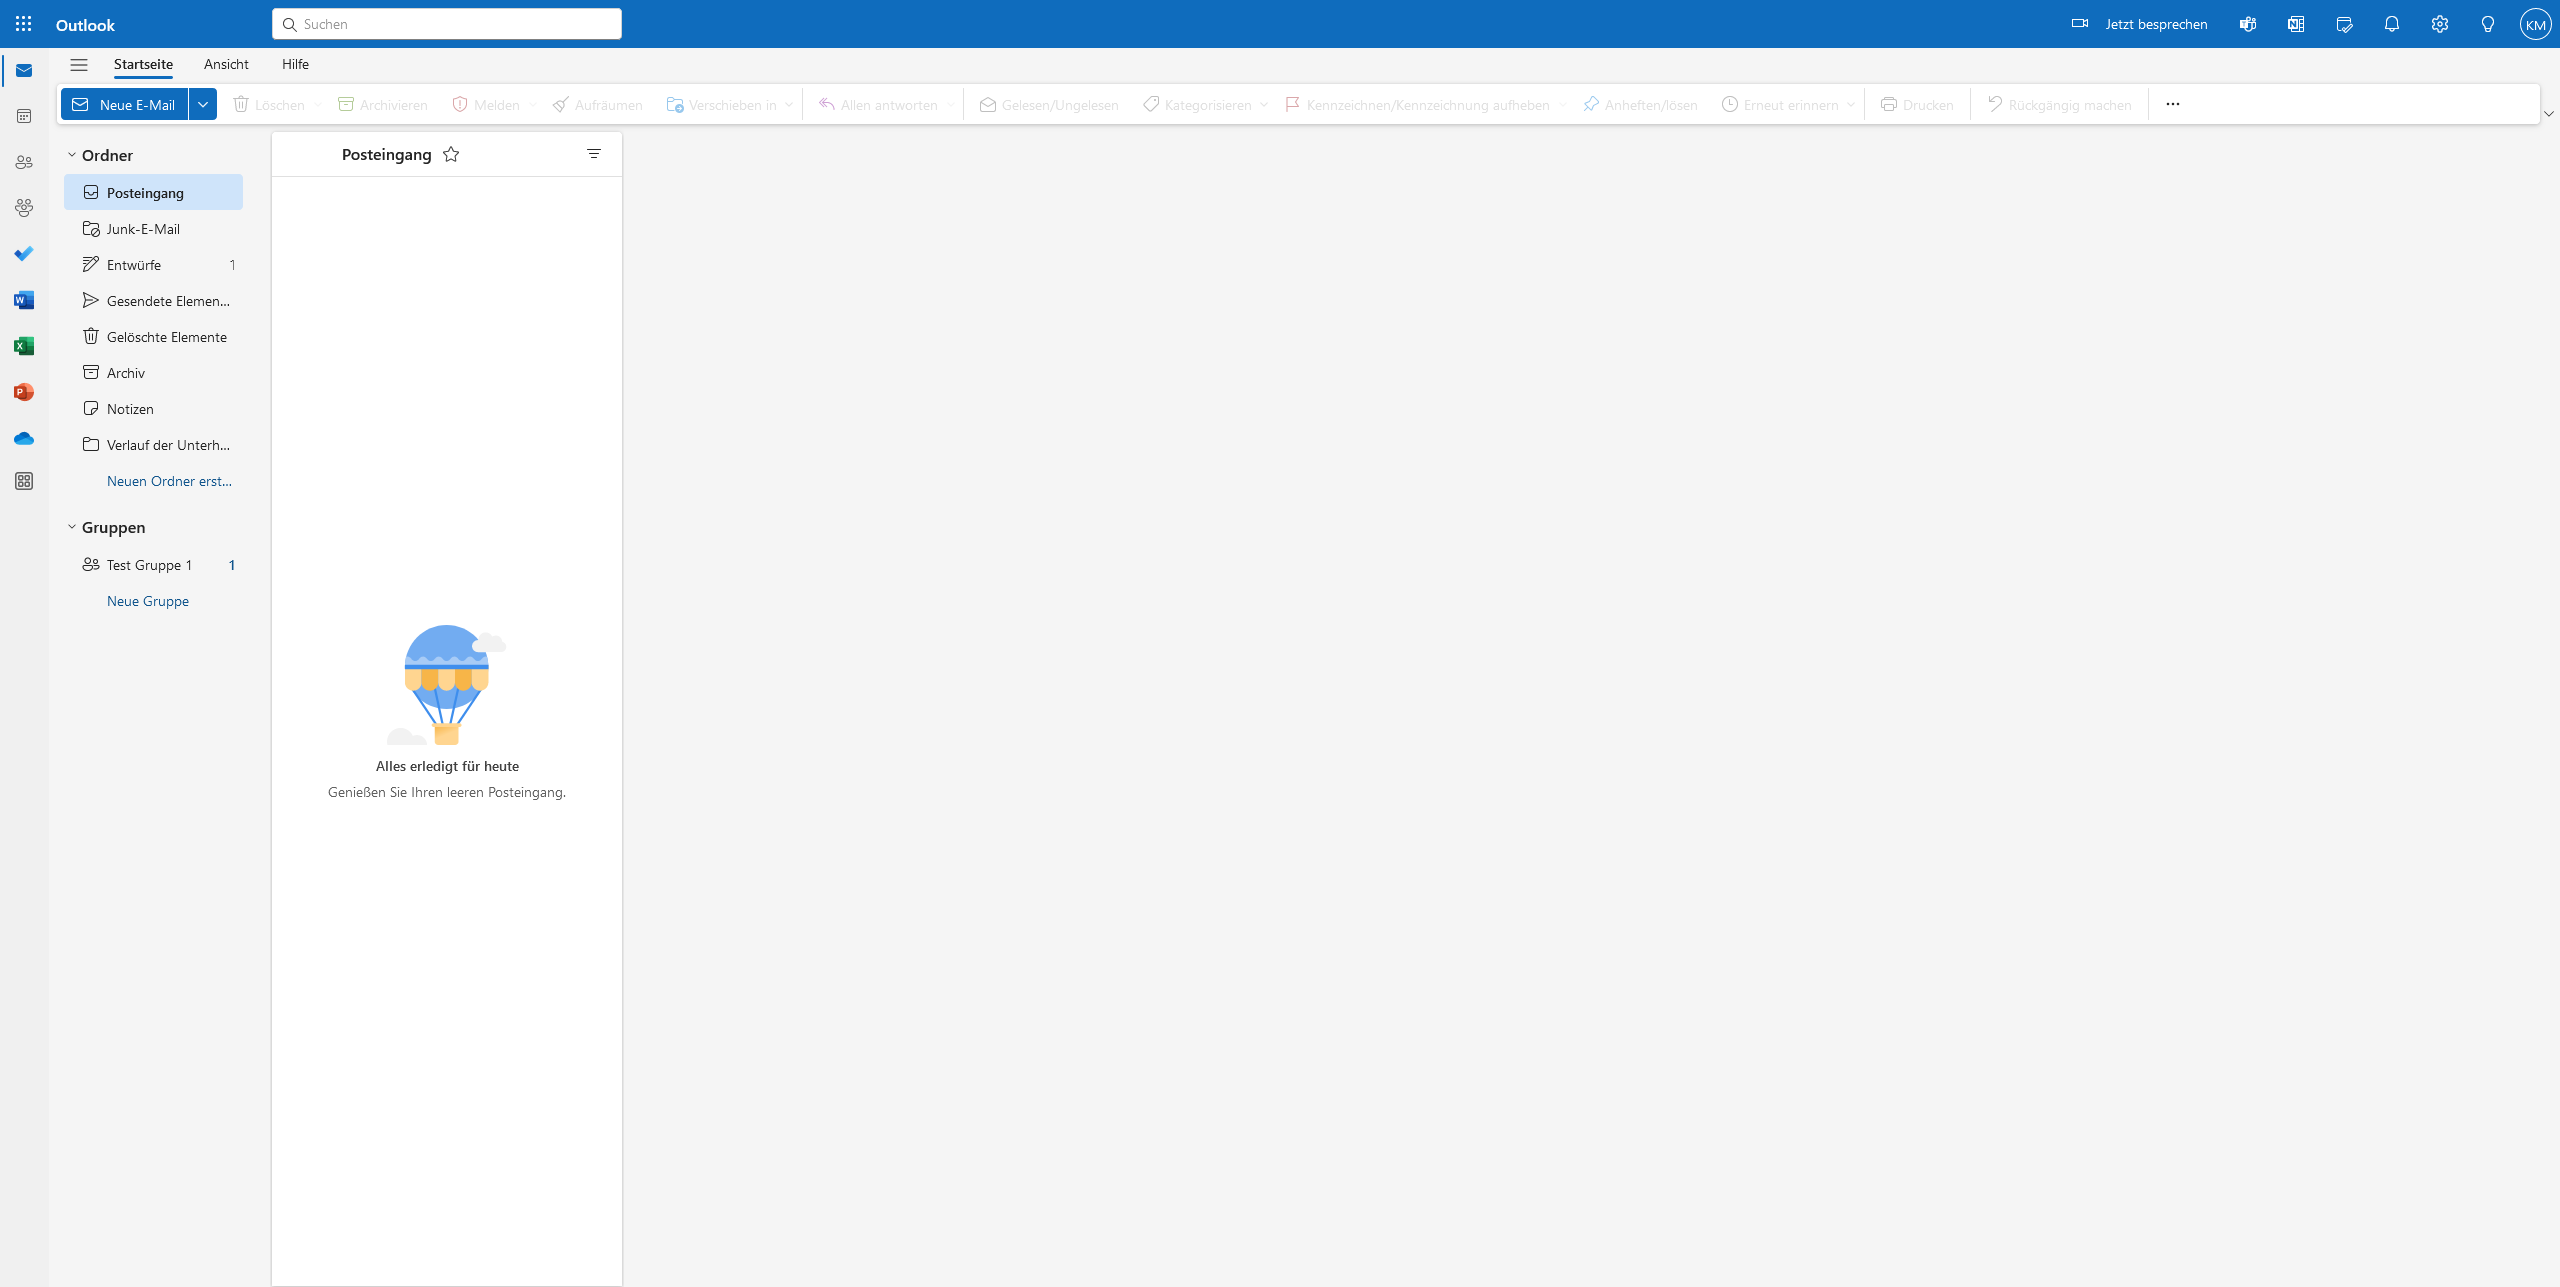
\includegraphics[width=0.75\textwidth]{images/OutlookLive_Mail1.png}
    \caption{OutlookLive Mail}
    \label{fig:outlook-live-mail}
\end{figure}

Die erste Hauptfunktion die Groupwaresysteme erfüllen ist das anbieten eines E-Mail Clients  über den E-Mails empfangen, versendet und verwaltet werden können.
Dabei sollten sich auch mehrere E-Mail Postfächer gleichzeitig hinzugefügt werden können.


\begin{figure}[H]
    \centering
    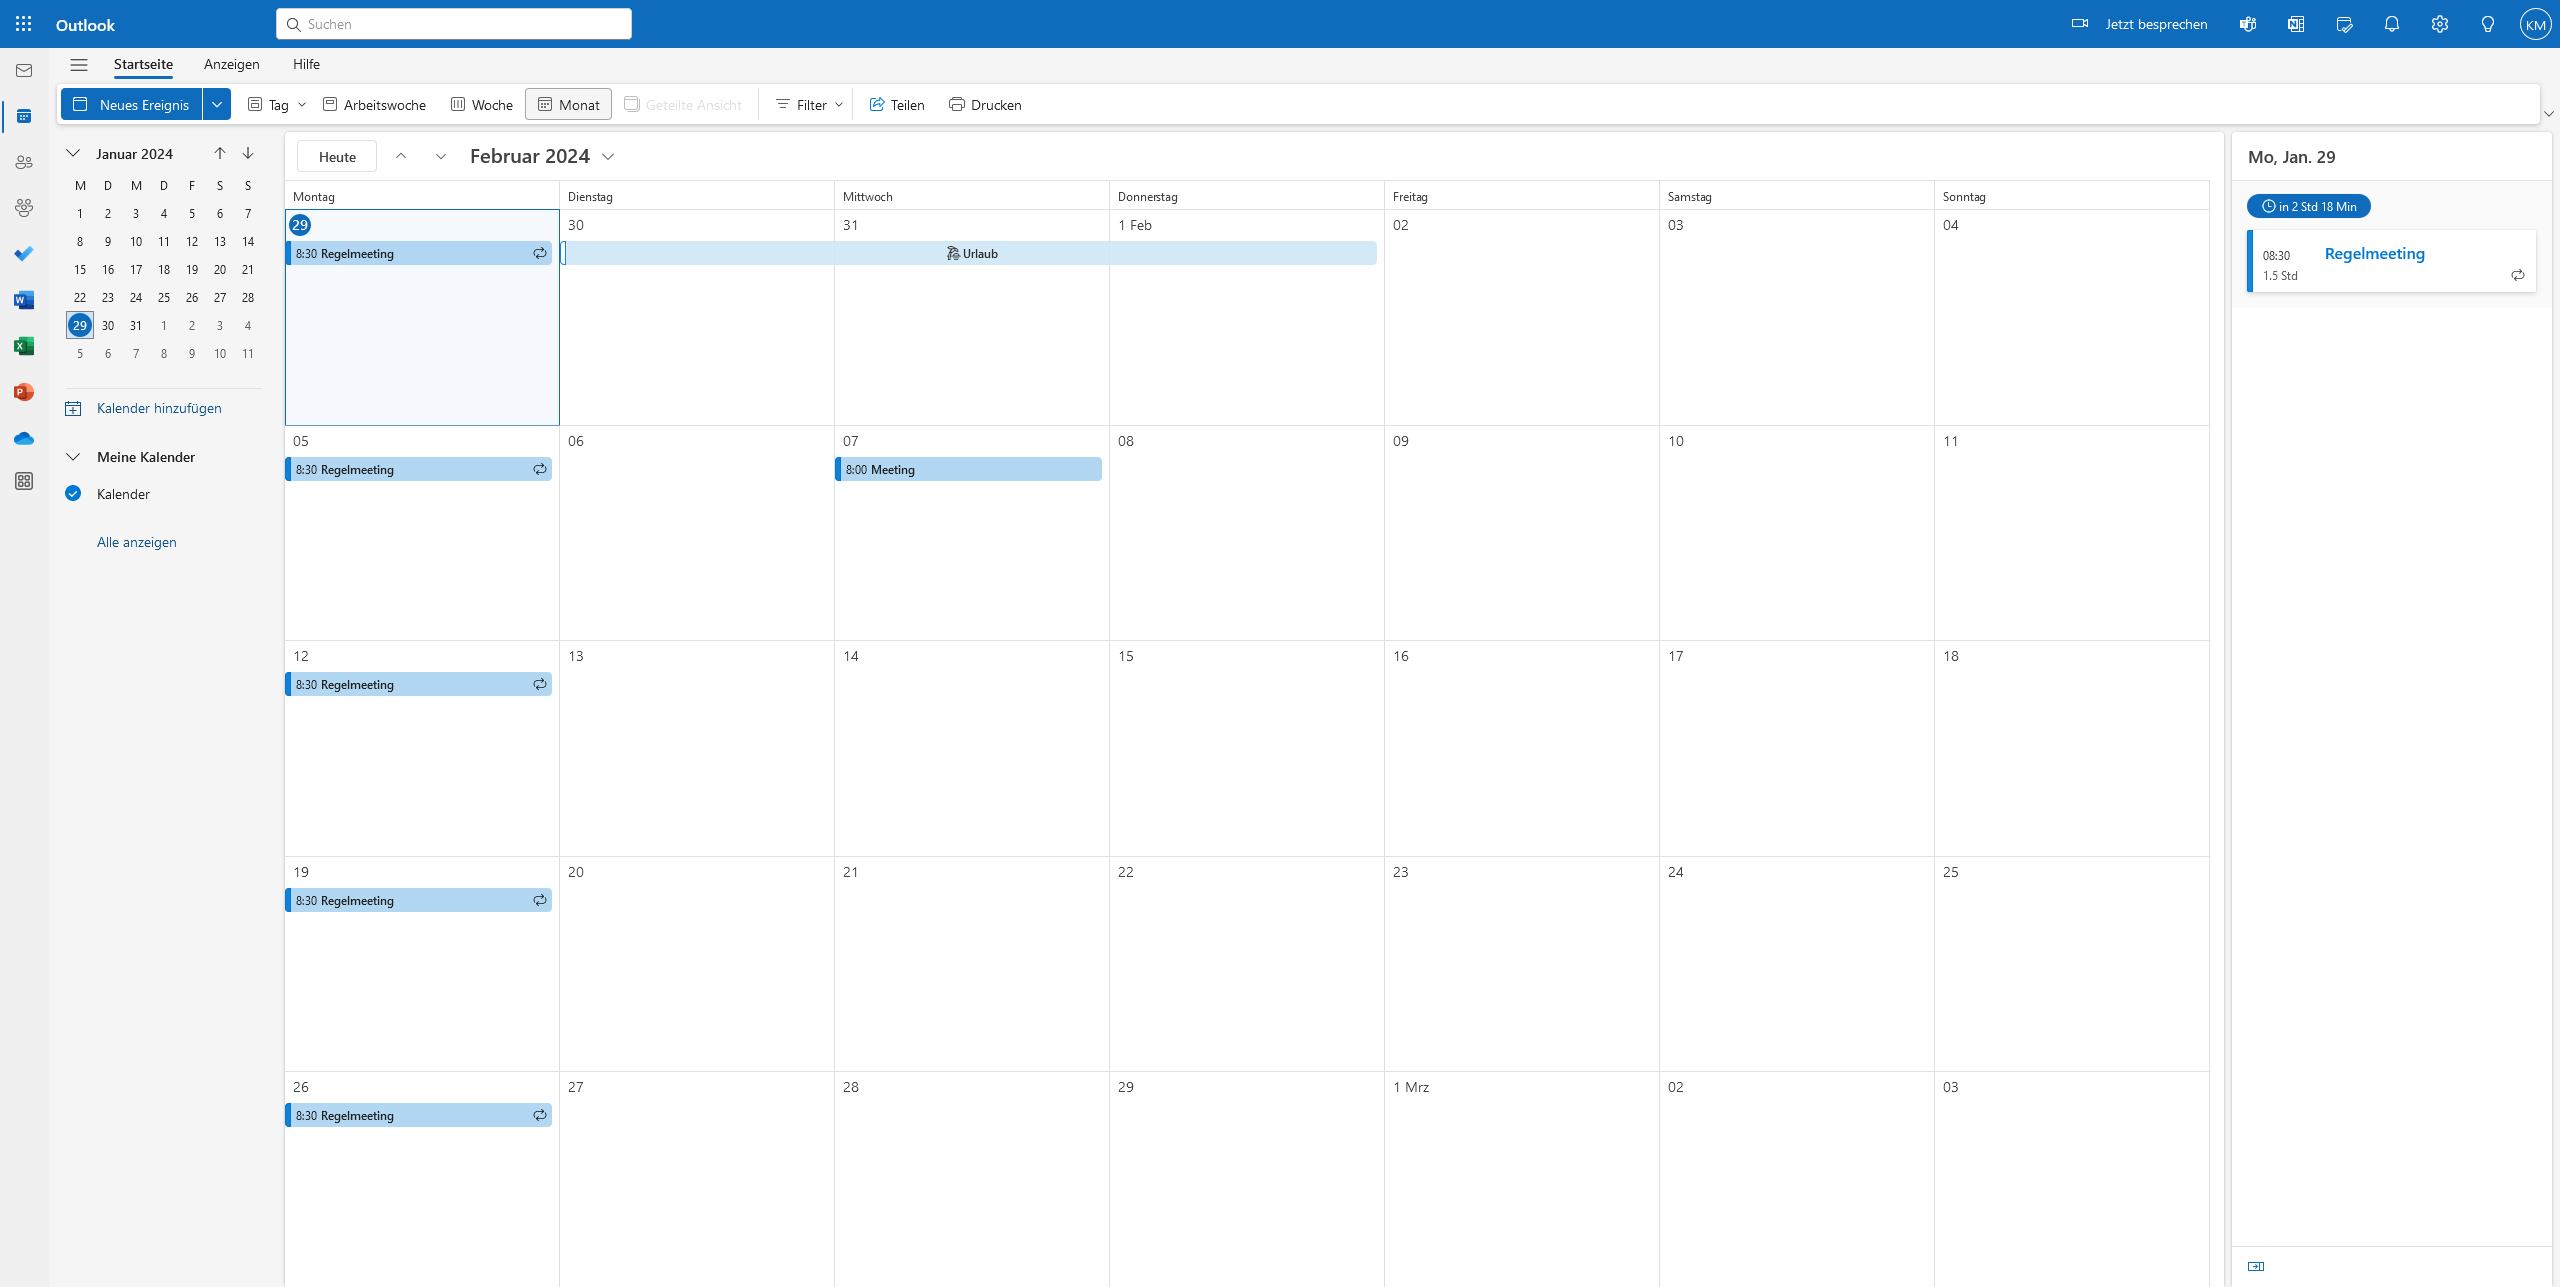
\includegraphics[width=0.75\textwidth]{images/OutlookLive_Calender1.png}
    \caption{OutlookLive Calender}
    \label{fig:outlook-live-calender}
\end{figure}

Eine weitere Hauptfunktion von Groupwaresystemen ist der Kalender, mit dem Terminplanung ermöglicht wird.
Die Terminplanung sollte zudem das Einladen von anderen Nutzern ermöglichen um die Zusammenarbeit und Organisation der Nutzer miteinander zu vereinfachen.
Dabei sollten auch Regeltermine, also Termine die sich regelmäßig wiederholen erstellt werden können.

\begin{figure}[H]
    \centering
    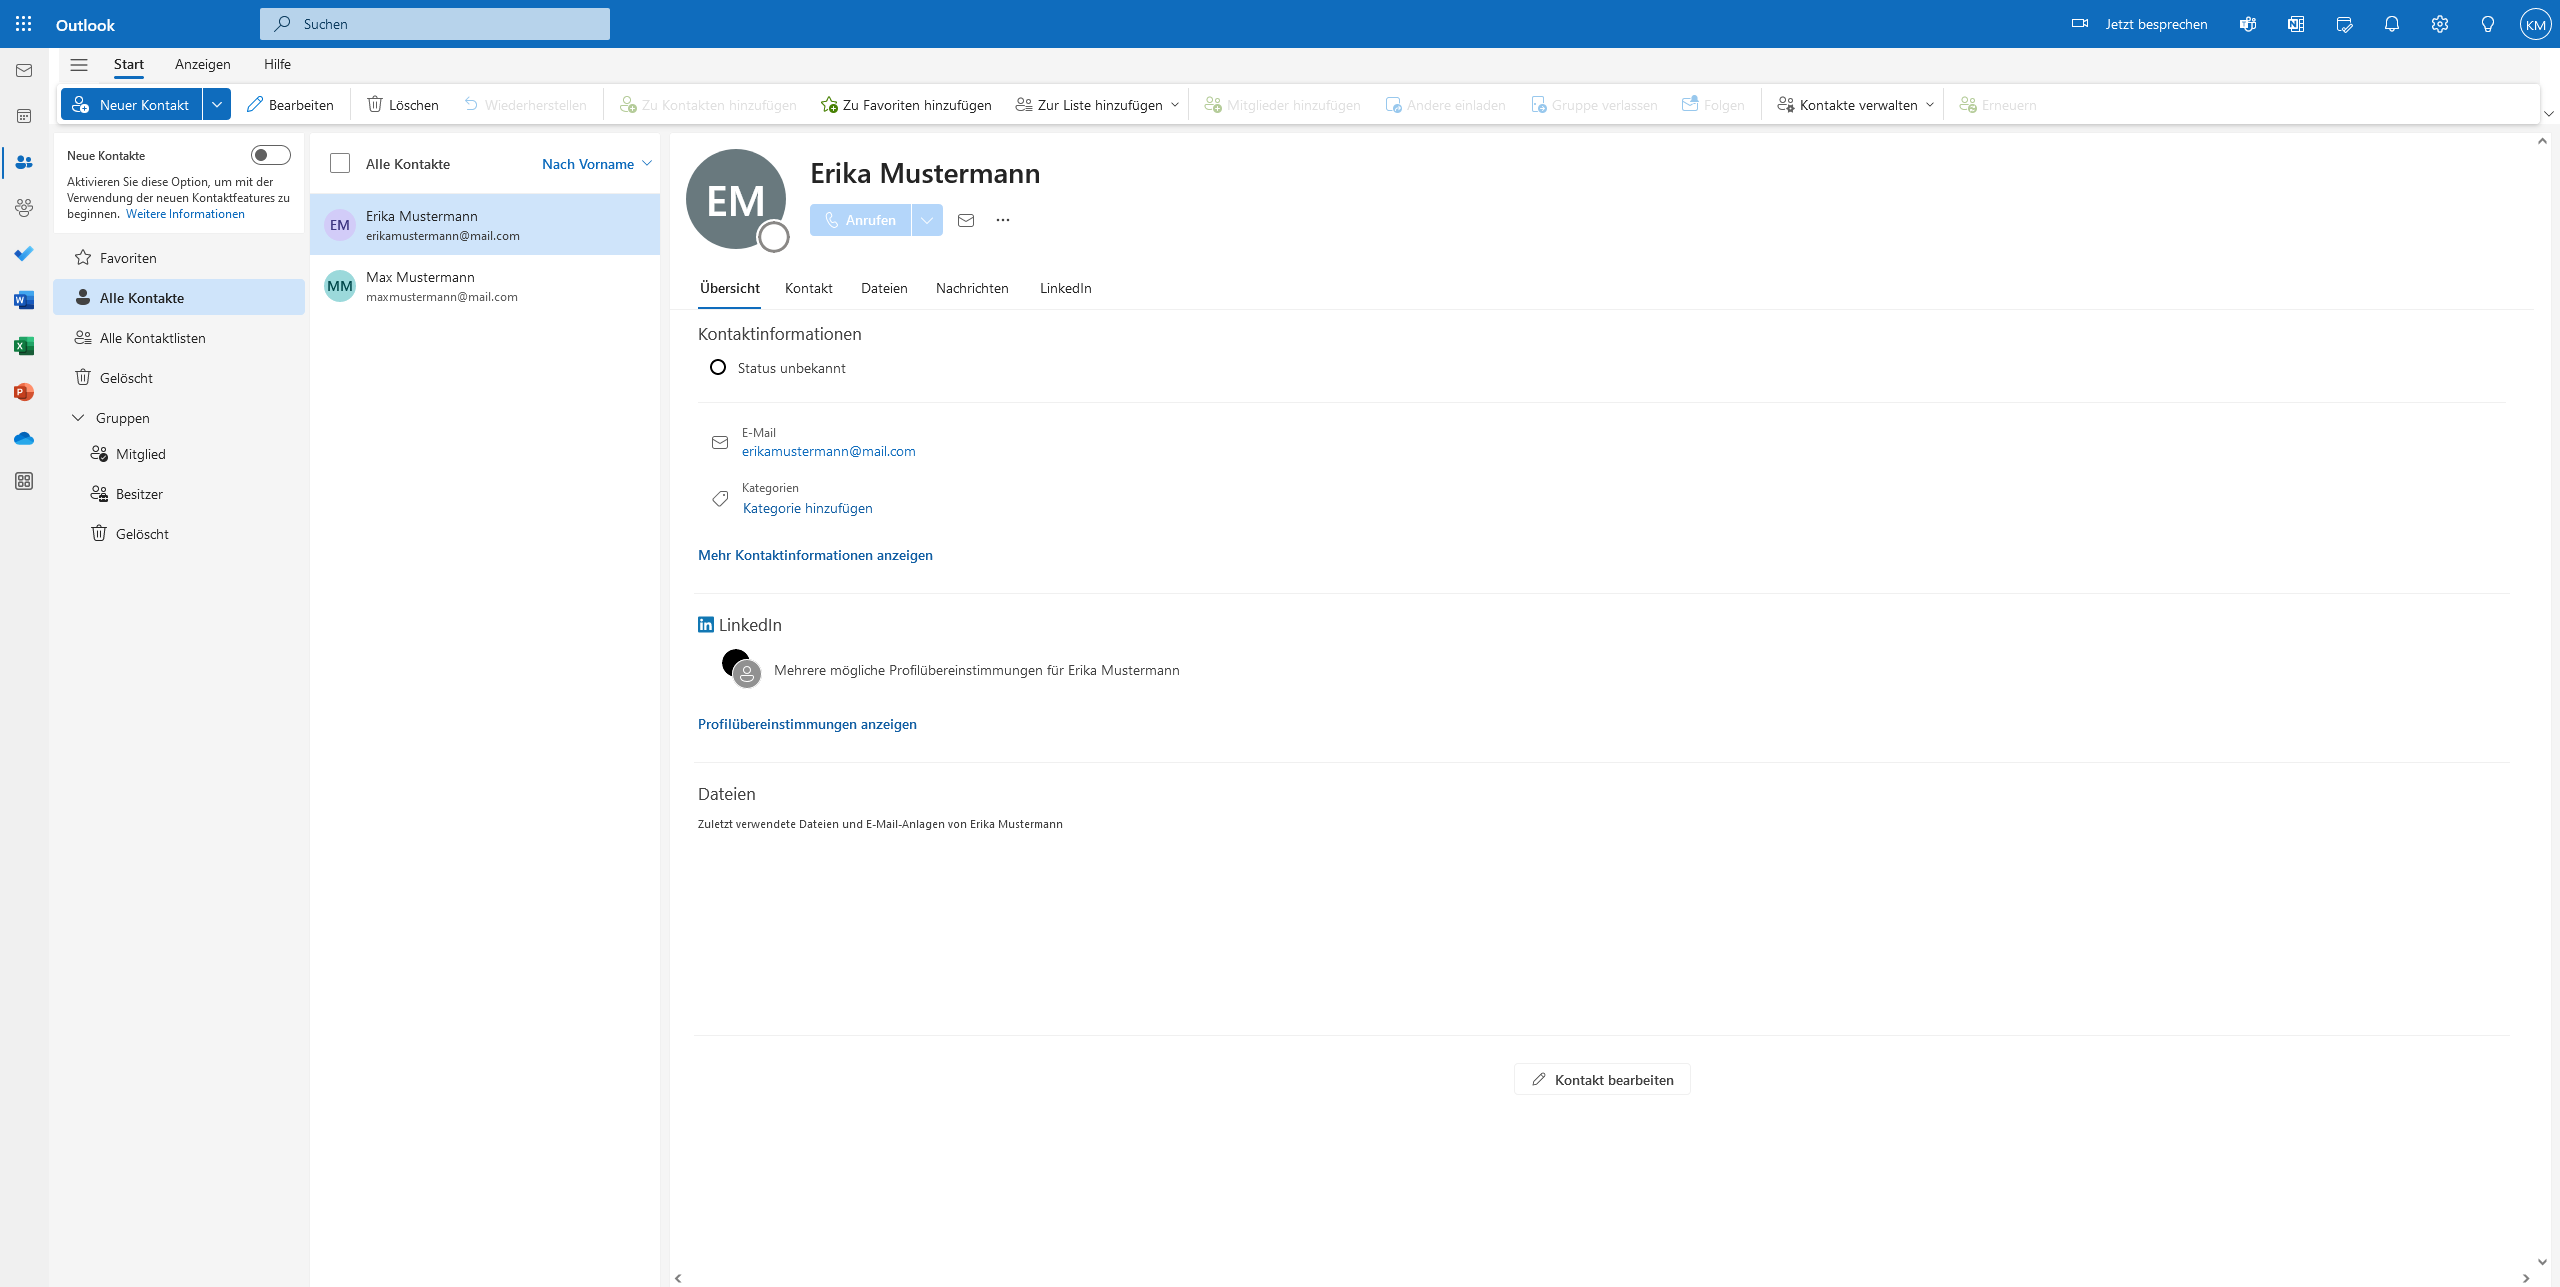
\includegraphics[width=0.75\textwidth]{images/OutlookLive_Contacts.png}
    \caption{OutlookLive Contacts}
    \label{fig:outlook-live-contacts}
\end{figure}

Kontakte sind eine esentieller Bestandteil von Groupwaresystemen um die Vernetzung innerhalb von Arbeitsgruppen zu organisieren.
Durch sie sollte die Kontaktaufnahme zu anderen Gruppenmitgliedern so einfach wie möglich gestaltet werden.
Im Beispiel von OutlookLive kann man beispielsweise wie in Abbildung \ref{fig:outlook-live-contacts} direkt vom Kontakt einer Person diese Person kontaktieren.


\section{Playwright}

Die Open-Source-Bibliothek Playwright wurde Anfang 2020 von Microsoft veröffentlicht und ermöglicht es, Browser automatisiert zu steuern und dadurch automatisierte Tests für Webanwendungen durchzuführen oder Websites zu scrapen.
Dabei bietet Playwright ein Application-Programming-Interface (API) für die Programmiersprachen JavaScript, TypeScript, Python, .NET und Java sowie eine Vielzahl von Funktionen, die das Testen von Webanwendungen erleichtern.
Beispielsweise kann mit Playwright Codegen die eigene Interaktion mit einer Webanwendung augezeichnet und als Code exportiert werden, der dann als Test für die ausgeführte Interaktion verwendet werden kann.
So können effizient Frontend-Tests für eine Vielzahl von Anwendungen implementiert werden.
\autocite[Quelle:][]{playwright}

Im Fall der Studienarbeit wurde Playwright verwendet, um automatisierte Tests für eine der recherchierten Groupware-Systeme durchzuführen.
Dabei werden Frontend-Tests implementiert, die typische Interaktionen mit der Benutzeroberfläche simulieren.
So können beispielsweise Formulare ausgefüllt oder Buttons angeklickt werden, womit ein Nutze-Login und das anschließende aufrufen der Mails des Nutzers simuliert werden kann.

Deckt man mit diesen Tests alle Funktionsbereiche des Groupwaresystems ab, kann man durch das Ausführen der Tests sicherstellen, dass die Anwendung nach einer Änderung noch wie erwartet funktioniert.
Auch falls die Anwendung in Zukunft unerwartete Ausfälle generiert, können diese durch die Tests schneller genauer erkannnt werden.
Geht beispielsweise der zuvor erwähnte Test des aufrufen der Mails schief, gibt es mit hoher Wahrscheinlichkeit ein Problem mit der Verbindung zum Mail Server.







\chapter{Recherche und Installation des Groupware-Systems}

In diesem Kapitel wird der Prozess der Recherche und Installation des Groupware-Systems beschrieben.
Dabei wird zuerst auf die Kriterien für das Groupware-System eingegangen, die im Laufe der Recherche berücksichtigt wurden.
Anschließend werden die betrachteten Groupware-Systeme vorgestellt und die Entscheidung für ein System begründet.
Zuletzt wird die Installation des Groupware-Systems auf einer Cloud-Instanz beschrieben.

\section{Kriterien für das Groupware-System}
\begin{itemize}
    \item \textbf{Open Source:} 
    Das erste und wichtigste Kriterium ist, dass das Groupware-System Open Source ist.
    Daher werden im Laufe der Recherche nur Open Source Groupware-Systeme betrachtet.
    \item \textbf{Eigenverwaltbarkeit:}
    Die Hochschule Esslingen hat ein eigenes Rechenzentrum und eine IT-Fakultät.
    Daher sollte die Software von der Hochschule Esslingen selbst installiert und administriert werden können.
    \item \textbf{Deutsche Firma:}
    Als deutsche Hochschule möchte die Hochschule Esslingen auch deutsche Firmen unterstützen.
    Deshalb ist es eine Vorgabe, dass das Groupware-System von einer deutschen Firma entwickelt wird.
    Dies ist zwar ein wichtiges Kriterium, muss aber nicht zwingend zum Ausschluss führen.
    \item \textbf{Automatisierbarkeit:}
    Teile der Konfiguration des Groupware-Systems, wie beispielsweise das Hinzufügen und die Konfiguration von Nutzern, sollen automatisierbar sein.
    Das soll das Hinzufügen und Entfernen der vielen Nutzer, die an der Hochschule Esslingen beschäftigt sind, erleichtern.
\end{itemize}

\newpage

\section{Betrachtete Groupware-Systeme}

Zu Beginn der Studienarbeit wurden anhand der gegebenen Kriterien mehrere Kandidaten für das Groupware-System recherchiert, um einen Überblick über die verfügbaren Möglichkeiten zu erhalten.
Im folgenden Abschnitt werden die 4 vielversprechendsten Groupware-Systeme der ersten Recherche, Kolab, Horde, Sogo und EGroupware, mit ihren Funktionalitäten und anderen relevanten Informationen vorgestellt.
Dabei wird auch auf die Verbreitung der Systeme an anderen Organisationen, vor allem aber Hochschulen und Universitäten, eingegangen.
Das soll eine erste Einschätzung über die Eignung der Systeme zur eigenen Verwaltung durch die Hochschule geben.


\subsection{Kolab}

Das Groupware-System Kolab wird von der Schweizer Firma Aphelia IT AG entwickelt und ist als Open-Source Produkt gratis verfügbar und bietet die folgenden Features:
\begin{itemize}
    \item E-Mail
    \item Kalender
    \item Kontakte
    \item Online-File-Server
    \item Aufgabenmanagement
    \item Notizen
    \item Sprach- und Videoanrufe
\end{itemize}
\autocite[Quelle:][]{kolab}

Kolab wird von der Firma Nestlé und der Universität Tübingen verwendet und ist daher auch für größere Organisationen geeignet.

\subsection{Horde}

Horde wird von einem gleichnamigen amerikanischen Unternehmen entwickelt und ist wie die anderen Systeme Open-Source und gratis verfügbar. Es bietet dabei die folgenden Funktionalitäten:
\begin{itemize}
    \item E-Mail
    \item Kalender
    \item Kontakte
    \item Online-File-Server
    \item Terminmanagement
    \item Projektmanagement
    \item Dokumentenmanagement
    
\end{itemize}
\autocite[Quelle:][]{horde}

Relevant für die Auswahl könnte auch sein, dass Horde schon von einigen anderen Universitäten und Hochschulen, wie beispielsweise der Universität Tübingen und Universität Paderborn, verwendet wird.

\subsection{Sogo}

Sogo ist ein Open-Source Groupware-System, welches von der französischen Firma Alinto entwickelt wird.
Das System ist frei verfügbar und bietet die folgenden Features:

\begin{itemize}
    \item E-Mail
    \item Kalender
    \item Kontakte
    \item Erinnerungen
    \item 2-Faktor-Authentifizierung
    \item Raum Reservationen
\end{itemize}
\autocite[Quelle:][]{sogo}

Ähnlich wie Horde wird auch Sogo von einigen Universitäten und Hochschulen verwendet, wie beispielsweise der Universität Koblenz und der Universität Ulm.

\subsection{EGroupware}

EGroupware ist ein Open-Source Groupware-System, welches von einer deutschen Firma entwickelt wird.

Als Funktionalitäten bietet EGroupware:

\begin{itemize}
    \item E-Mail
    \item Kalender
    \item Kontakte
    \item Online-File-Server
    \item Terminmanagement
    \item Projektmanagement
    \item Dokumentenmanagement
\end{itemize}

Auch EGroupware wird von einigen Hochschulen genutzt, jedoch von deutlich weniger als die anderen Systeme.


\section{Entscheidung für ein Groupware-System}

Bei der Recherche der verschiedenen Groupware-Systeme wurde klar, dass alle der untersuchten Systeme die grundlegenden gewünschten Funktionalitäten bieten und daher grundsätzlich alle für die Hochschule Esslingen geeignet sind.
Durch diesen Umstand konnte die Entscheidung nicht rein aufgrund der Funktionalitäten der Systeme getroffen werden, da sich keines der Systeme in diesem Punkt stark von den anderen abhebt.
Somit fiel final die Entscheidung auf EGroupware, da es von einer deutschen Firma entwickelt wird und umfangreiche Funktionen bietet, die für die Hochschule Esslingen relevant sein könnten.




\section{Installation auf der Cloud}

Für die Installation der EGroupware Software stellt die EGroupware GmbH eine Installationsanleitung zu Verfügung.
Darin wird auf einer Linux Instanz zunächst ein Docker Repository hinzugefügt und anschließend die EGroupware Software in Form von 5 Docker Containern installiert und gestartet.
Alle dafür benötigten Konsolenbefehle waren in der Installationsanleitung angegeben. \autocite{egroupware-installation}

Für das Hosting der EGroupware Software wurde sowohl WSL2 (Windows-Subsystem für Linux) als auch eine bwCloud Instanz getestet.
Die reine Installation der Software verlief auf beiden Systemen auf einer Ubuntu22.04 Instanz ohne Probleme.
Im Laufe der Konfiguration wurde jedoch klar, dass die Netzwerkkonfiguration bei bwCloud einfacher zu handhaben ist als bei WSL2.
Daher wurde die finale Installation und Konfiguration auf einer bwCloud Instanz durchgeführt.
Damit das Frontend der Software über das Internet erreichbar ist, muss Port 80 für HTTP Kommunikation freigegeben werden.
Das wurde wie in Abbildung \ref{fig:bwcloud_security_group} gezeigt in einer benutzerdefinierten Sicherheitsgruppe der bwCloud Instanz realisiert.
\begin{figure}[H]
    \centering
    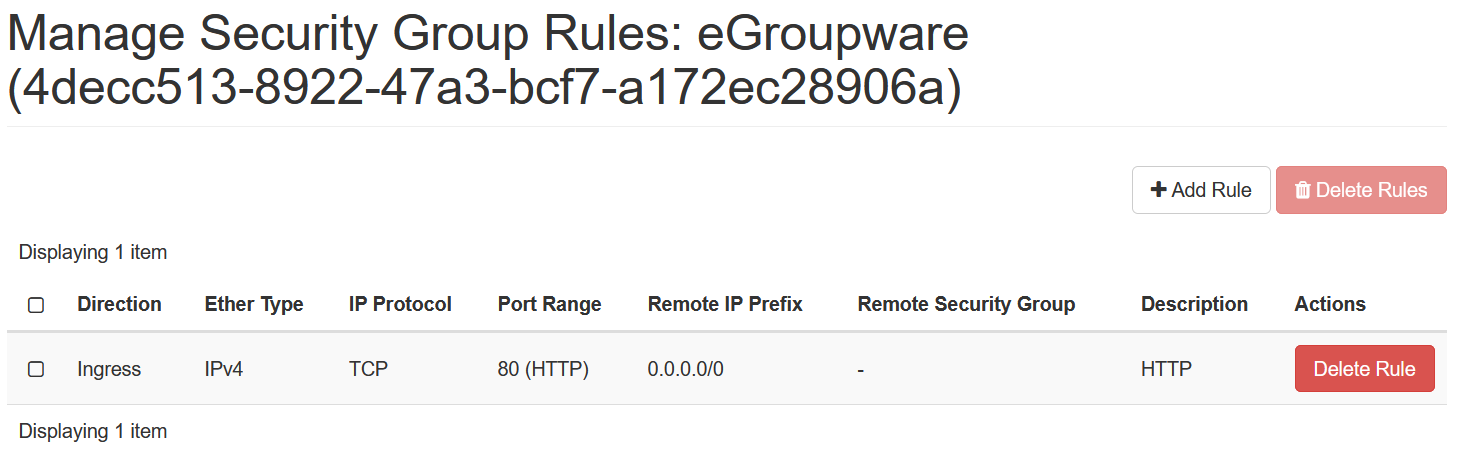
\includegraphics[width=0.75\textwidth]{images/bwCloud_SecurityGroup.png}
    \caption{Konfiguration der Sicherheitsgruppe für die bwCloud Instanz von EGroupware}
    \label{fig:bwcloud_security_group}
\end{figure}

Für die grundlegende Konfiguration der Software, wie beispielsweise das Konfigurieren von LDAP oder SAML 2.0, bietet die EGroupware Software ein Setup-Tool, welches über folgende URL erreichbar ist:

\fbox{\texttt{http://host-or-ip/egroupware/setup/}}

Für den ersten Zugriff auf die tatsächliche Software für beispielsweise das Erstellen von Nutzer Accounts wird bei der Installation automatisch ein Administrator Account angelegt, dessen Zugangsdaten im Log der Installation zu finden sind.
Das Frontend der Groupware ist dann über die folgende URL erreichbar:

\fbox{\texttt{http://host-or-ip/egroupware/login.php/}}


\chapter{Testing von EGroupware mit Playwright}

Nach erfolgreicher Installation von EGroupware kann das System nun über jeden Browser aufgerufen werden und kann daher getestet werden.
Dabei wird das System mit Hilfe von Playwright getestet.

\section{Aufsetzen der Testumgebung}

Für das entwickeln der Tests wird die Entwicklungsumgebung Visual Studio Code verwendet da es durch  Erweiterung "Playwright Test for VSCode" von Microsoft eine sehr gute Integration der Playwright API bietet.
Mit dieser Erweiterung kann auch die vollständige Installation von Playwright in dem aktuellen Projektordner direkt in der Entwicklungsumgebung durchgeführt werden.
Durch diese Installation wird ein Beispieltest erstellt welcher als Vorlage für weitere Tests genutzt werden kann.
Für das Testen der meisten Funktionen der EGroupware Anwendung wird der Administrator Account genutzt, der automatisch bei der Installation erstellt wird.
Dafür wird der Nutzername und das Passwort des Administrators in der Test Datei als Objekt gespeichert und kann dann in den Tests genutzt werden.
Außerdem wurde diesem Account eine E-Mail Adresse über IMAP hinzugefügt, damit auch die E-Mail Funktion getestet werden kann.

\section{Implementierung der Tests}

Alle Tests werden in TypeScript geschrieben und können daher direkt in der Entwicklungsumgebung ausgeführt werden.
Dabei werden alle Tests in dieser Studienarbeit in einem Chromium Browser ausgeführt.


\subsection{Login}

Da alle Tests der Anwendung einen eingelogten Nutzer benötigen wird zuerst ein Login Test implementiert, der ein Nutzerobjekt mit Nutzernamen und Passwort erhält und sich dann versucht in der Anwendung einzuloggen.
Dieser Test wird zu Beginn jedes anderen Tests ausgeführt um den Nutzer einzuloggen.

\subsection{Aufrufen einer Email}

Dieser Test ist sehr selbsterklärend.
Er versucht sich als der Administrator einzuloggen und ruft dann die erste E-Mail in der E-Mail Liste auf.
Dabei wird die Verbindung der Groupware zum IMAP Server getestet.

\subsection{Erstellen eines Termins}

Beim Test zum Erstellen eines Termins wird sich als Administrator eingeloggt und dann ein Termin erstellt.
Die Daten für diesen Termin sind ähnlich wie die Daten für den Login mit dem Administrator Account in einem Objekt gespeichert und können so einfach in den Test eingefügt werden.
Jedoch wird dieses Objekt erst beim ausführen des Tests erstellt, da das Datum für den Termin immer das aktuelle Datum sein soll und daher nicht statisch in einem globalen Objekt gespeichert werden kann.
Dafür wird mit  Hilfe des Timestamp der Funktion Date.now() ein Datum erstellt, welches dann in einen String umgewandelt wird und in das Objekt gespeichert wird.
So kann jederzeit ein Termin erstellt werden, welcher 30 Minuten nach der Ausführung des Tests stattfindet.

\subsection{Erstellen und Löschen eines neuen Nutzers}

Der letzte Test der in dieser Studienarbeit implementiert wurde ist ein Test zum Erstellen eines Nutzers, der sich anschließend mit dem neuen Nutzer einloggt und ihn daraufhin wieder löscht.
Auch hier werden die Daten für den neuen Nutzer in einem Objekt gespeichert, welches dann in den Test eingefügt wird und später fürs einloggen mit dem Nutzer genutzt wird.
Mit diesem Test soll die Backend-Funktionalität des Nutzermanagements getestet werden.

\section{Ausführen der Tests}




% Eigenkorrekturlesung 1 fertig
\chapter{Zusammenfassung}

In diesem Kapitel wird ein Fazit über den Verlauf des Studienprojekts und das im Rahmen des Studienprojekts untersuchte Groupware-System als Lösung für die Hochschule Esslingen gezogen.
Zuletzt wird ein Ausblick auf mögliche nächste Schritte in der Suche nach einer Groupware-Lösung für die Hochschule Esslingen gegeben.

\section{Fazit}

Das Ziel des Studienprojekts war es, ein Groupware-System zu finden und zu testen, das die Anforderungen der Hochschule Esslingen erfüllt.
Dabei wurden die Anforderungen an das Groupware-System in einem ersten Schritt definiert und anschließend die verfügbaren Groupware-Systeme recherchiert.
Nachdem das Groupware-System ausgewählt wurde, wurde es auf einer Cloud-Instanz installiert und konfiguriert.
Zuletzt wurden automatisierte End-to-End-Tests für das Groupware-System implementiert und durchgeführt.

Das Ziel des Studienprojekts wurde insofern erreicht, als dass ein erstes Groupware-System installiert und getestet wurde.
Das untersuchte Groupware-System, EGroupware, erfüllt dabei die funktionalen Anforderungen der Hochschule an ein Groupware-System, wie E-Mails, Kalender mit Terminplanung und Kontakte.
Auch die nicht-funktionale Anforderung der Eigenadministration wurde erfüllt, da die Installation und Konfiguration des Systems auf einer Cloud-Instanz durchgeführt werden konnte.

Ein Faktor, bei dem bei EGroupware noch Zweifel aufwirft, ist die Möglichkeit zur Automatisierung von Teilen des Systems.
Da bei Tests mit Playwright zum Erstellen und Löschen von Nutzern Asynchronitäten in den angezeigten Nutzeraccounts auftraten, ist in Frage zu stellen, ob das System für ausführliche Automatisierung geeignet ist.
Daher kann ohne weitere ausführliche Tests noch nicht eindeutig gesagt werden, ob EGroupware die Anforderungen der Hochschule Esslingen aus den recherchierten Groupware-Systemen am besten erfüllt.


\section{Ausblick}

In diesem Studienprojekt wurde die Basis der Suche nach einem neuen Groupware-System für die Hochschule Esslingen gelegt.
Dabei wurden die Anforderungen an das Groupware-System definiert und ein erstes Groupware-System installiert und getestet.

Im nächsten Schritt soll, möglicherweise in weiteren Studienprojekten, die Recherche nach einem Groupware-System mit der Installation und dem Testen weiterer Groupware-Systeme fortgesetzt werden.
Alle der in diesem Studienprojekt betrachteten Groupware-Systeme erfüllen die grundsätzlichen Anforderungen der Hochschule an ein neues Groupware-System.
Daher könnte es sinnvoll sein, in Zukunft noch Kolab, Horde und Sogo, die bereits von deutlich mehr Hochschulen genutzt werden als EGroupware, als mögliche Lösungen für die Hochschule Esslingen zu betrachten.

Falls EGroupware weiterhin als Lösung für die Hochschule Esslingen in Betracht gezogen wird, sollte die mögliche Automatisierung von Teilen des Systems genauer untersucht werden.
Beispielsweise sollte die Robustheit des Systems beim Erstellen vieler Nutzer auf einmal getestet werden, um sicherzustellen, dass das System die Anforderungen der Hochschule Esslingen erfüllt.




\printbibliography


\end{document}